\graphicspath{{./figures/capitolo5/}}
\lstset{inputpath = ./programs/capitolo5}
\pgfplotstableset{search path = ./tables/capitolo5}

\chapter{Sistemi lineari di equazioni}

Questo capitolo è dedicato interamente ai sistemi dinamici lineari,
con particolare attenzione al caso dei sistemi dinamici \emph{positivi}.
Dopo una breve introduzione teorica, passeremo all'analisi
di alcuni modelli, sia discreti che continui.

\section{Sistemi di equazioni differenziali}

Consideriamo la funzione di matrice $\exp(At)$.
Dato che la funzione esponenziale è sufficientemente regolare,
il Teorema \ref{teor:funzione-di-matrice-derivata} ci dice che
\[
\frac{d}{dt} e^{At} = A e^{At},
\]
quindi è immediato verificare che la funzione $y(t) = \exp(At)y_0$
risolve il problema di Cauchy
\begin{equation}
\left\{
\begin{aligned}
y'(t)  &= Ay(t) \quad \text{per ogni $t \geq t_0$}, \\
y(t_0) &= y_0 \in \R^m.
\end{aligned}
\right.
\end{equation}
Questo tipo di ragionamento, che generalizza la teoria scalare al caso
vettoriale per mezzo delle funzioni di matrice, può essere esteso anche
al caso non omogeneo e non autonomo: vediamo come.
Consideriamo il problema di Cauchy
\begin{equation}\label{eq:problema-lineare-continuo}
\left\{
\begin{aligned}
y'(t)  &= A(t)y(t) + b(t) \quad \text{per ogni $t \geq t_0$}, \\
y(t_0) &= y_0 \in \R^m,
\end{aligned}
\right.
\end{equation}
con $A(t), b(t)$ funzioni sufficientemente regolari del tempo $t$
(eventuali derivate e integrali sono da intendersi componente per componente).

\begin{teor}
Sia $W(t)$ la funzione a valori matriciali tale che
\[
\left\{
\begin{aligned}
& W'(t) = A(t) W(t) \quad \text{per ogni $t \geq t_0$}, \\
& W(t_0) \in \R^{m \times m} \quad \text{è invertibile}.
\end{aligned}
\right.
\]
Allora $W(t)$ è invertibile per ogni $t \geq t_0$.
\end{teor}

\begin{defi}[Matrice fondamentale]
Si dice \emph{matrice fondamentale} del problema \eqref{eq:problema-lineare-continuo}
la funzione a valori matriciali $\Phi(t,s) = W(t)W^{-1}(s)$,
definita per ogni $t,s \geq t_0$.
\end{defi}

\begin{teor}
La definizione di $\Phi(t,s)$ non dipende da $W(t_0)$.
Inoltre, $\Phi(t,s) \Phi(s,r) = \Phi(t,r)$ per ogni $r,s,t \geq t_0$
e $\Phi(t,s)^{-1} = \Phi(s,t)$ per ogni $s,t \geq t_0$.
La matrice fondamentale $\Phi(t,t_0)$ con $t_0$ fissato è soluzione
del problema di Cauchy
\[
\left\{
\begin{aligned}
& \frac{d}{dt} \Phi(t,t_0) = A(t) \Phi(t,t_0) \quad \text{per ogni $t \geq t_0$}, \\
& \Phi(t_0,t_0) = I \in \R^{m \times m}.
\end{aligned}
\right.
\]
Nel caso in cui $A(t) \equiv A$, si ha che $\Phi(t,s) = e^{A(t-s)}$.
\end{teor}

\begin{teor}
Il problema di Cauchy \eqref{eq:problema-lineare-continuo} ha come soluzione
\begin{equation}  \label{eq:soluzione-problema-lineare-continuo}
y(t) = \Phi(t,t_0) y_0 + \int_{t_0}^t \Phi(t,s) b(s) \ds.
\end{equation}
Se il problema è autonomo, la formula si semplifica in
\begin{equation} \label{eq:soluzione-problema-lineare-autonomo-continuo}
y(t) = e^{A(t-t_0)} y_0 + \left( \int_0^{t-t_0} e^{As} \ds \right) b.
\end{equation}
\end{teor}

L'esistenza di queste formule chiuse riassume vantaggi e svantaggi
dell'uso di modelli lineari piuttosto che modelli non lineari:
i primi sono più semplici da analizzare e da simulare, ma i secondi
hanno dinamiche potenzialmente più ricche (vedremo degli esempi
nel prossimo capitolo). Queste formule sono inoltre importanti
perché consentono non solo di descrivere la dinamica di un sistema
lineare in un intervallo di tempo limitato $[t_0,T]$, ma anche la
dinamica per tempi lunghi $t \to \infty$. Sono molte infatti le applicazioni
in cui non è tanto la dinamica \emph{transiente} a essere importante,
quanto quella \emph{asintotica}. Approfondiamo quest'ultimo aspetto
nel caso autonomo:

\begin{defi}
Ogni punto $\bar{y} \in \R^m$ tale che $0 = A\bar{y} + b$ è detto
\emph{punto di equilibrio} per l'equazione differenziale
$y'(t) = A y(t) + b$, perché è immediato verificare che $y(t) \equiv \bar{y}$
è una soluzione costante dell'equazione.
\end{defi}

\begin{teor} \label{teor:dinamica-asintotica-lineare-continuo}
Se $A$ è invertibile, esiste ed è unico un punto di equilibrio $\bar{y}$ per
l'equazione differenziale $y'(t) = A y(t) + b$, e il problema ai valori
iniziali associato (con $y(t_0) = y_0$) ha soluzione
\begin{equation} \label{eq:soluzione-problema-lineare-autonomo-Ainv-continuo}
y(t) = e^{A(t-t_0)} (y_0 - \bar{y}) + \bar{y}.
\end{equation}
Per quanto riguarda la dinamica asintotica, a meno che $y_0 = \bar{y}$,
ci sono tre possibilità:
\begin{itemize}
\item $y(t) \to \bar{y}$ se e solo se $\sigma(A) \subseteq \C^-$.
	In questo caso il problema si dice \emph{dissipativo} e il punto di
	equilibrio $\bar{y}$ si dice \emph{asintoticamente stabile}.
\item $y(t)$ rimane in un intorno limitato di $\bar{y}$ per ogni $t \geq t_0$
	se e solo se $\Re(\lambda) \leq 0$ per ogni $\lambda \in \sigma(A)$, e in più
	ogni autovalore puramente immaginario di $A$ è semisemplice.
	In questo caso il punto di equilibrio $\bar{y}$ si dice \emph{stabile}.
\item $\norm{y(t)} \to +\infty$ se e solo se non è verificata la condizione
	del punto precedente. In questo caso il punto di equilibrio $\bar{y}$
	si dice \emph{instabile}.
\end{itemize}
\end{teor}

\begin{proof}
Se $A$ è invertibile, si ha necessariamente che $\bar{y} = -A^{-1}b$.
La formula \eqref{eq:soluzione-problema-lineare-autonomo-Ainv-continuo}
si dimostra facilmente a partire dalla
\eqref{eq:soluzione-problema-lineare-autonomo-continuo} osservando che
$A^{-1}e^{As}$ è una primitiva di $e^{As}$ e utilizzando il teorema
fondamentale del calcolo integrale. La descrizione della dinamica asintotica
si ottiene applicando il Teorema \eqref{teor:andamento-asintotico-esponenziale-matrice}
alla funzione di matrice presente nella formula
\eqref{eq:soluzione-problema-lineare-autonomo-Ainv-continuo}.
\end{proof}

\section{Sistemi di equazioni alle differenze}

La teoria nel caso discreto ricalca perfettamente quella del caso continuo.
Consideriamo il problema di Cauchy
\begin{equation} \label{eq:problema-lineare-discreto}
\left\{
\begin{aligned}
y_{n+1} &= A_n y_n + b_n \quad \text{per ogni $n \geq n_0$}, \\
y_{n_0} &= y_0 \in \R^m,
\end{aligned}
\right.
\end{equation}
con $A_n$ matrice invertibile per ogni $n \geq n_0$.

\begin{teor}
Sia $\Phi_{n,k} = \bigl( \prod_{i=n_0}^{n-1} A_i \bigr)
\bigl( \prod_{i=n_0}^{k-1} A_i^{-1} \bigr)$ per ogni $n,k \geq n_0$.
Allora il problema \eqref{eq:problema-lineare-discreto} ha soluzione
\[
y_n = \Phi_{n,n_0} y_0 + \sum_{k=n_0}^{n-1} \Phi_{n,k+1} b_k.
\]
Se il problema è autonomo, cioè $A_n \equiv A$ e $b_n \equiv b$, la formula
si semplifica:
\[
y_n = A^{n-n_0} y_0 + \left( \sum_{k=0}^{n-n_0-1} A^k \right) b.
\]
\end{teor}

\begin{teor} \label{teor:dinamica-asintotica-lineare-discreto}
Se $A-I$ è invertibile, esiste ed è unico un punto di equilibrio $\bar{y}$ per
l'equazione alle differenze $y_{n+1} = A y_n + b$, e il problema ai valori
iniziali associato (con $y_{n_0} = y_0$) ha soluzione
\begin{equation} \label{eq:soluzione-problema-lineare-autonomo-AIinv-discreto}
y_n = A^{n-n_0} (y_{n_0} - \bar{y}) + \bar{y}.
\end{equation}
Per quanto riguarda la dinamica asintotica, a meno che $y_0 = \bar{y}$,
ci sono tre possibilità:
\begin{itemize}
\item $y_n \to \bar{y}$ se e solo se $\abs{\lambda} < 1$ per ogni
	$\lambda \in \sigma(A)$. In questo caso il problema si dice \emph{dissipativo}
	e il punto di equilibrio $\bar{y}$ si dice \emph{asintoticamente stabile}.
\item $y_n$ rimane in un intorno limitato di $\bar{y}$ per ogni $n \geq n_0$
	se e solo se $\abs{\lambda} \leq 1$ per ogni $\lambda \in \sigma(A)$,
	e in più ogni autovalore di $A$ sul bordo del disco unitario è semisemplice.
	In questo caso il punto di equilibrio $\bar{y}$ si dice \emph{stabile}.
\item $\norm{y_n} \to +\infty$ se e solo se non è verificata la condizione
	del punto precedente. In questo caso il punto di equilibrio $\bar{y}$
	si dice \emph{instabile}.
\end{itemize}
\end{teor}

\section{Sistemi dinamici positivi}

Nelle applicazioni capita spesso di avere a che fare con modelli che descrivono
l'evoluzione di grandezze reali il cui segno è noto a priori (tipicamente positivo):
si pensi, ad esempio, al numero di individui in una popolazione, alla probabilità
che accada un certo evento, alla concentrazione di un reagente chimico, ecc.
In tutti questi casi, l'ipotesi di segno costante (d'ora in poi positivo,
senza perdita di generalità) può essere sfruttata per ottenere risultati
ancora più forti di quelli visti nei paragrafi precedenti, soprattutto per
quanto riguarda la caratterizzazione dei punti di equibrio $\bar{y}$.
Prima di passare alla teoria per sistemi dinamici, riportiamo innanzitutto
alcuni risultati di base sulle \emph{matrici positive} e sulle \emph{M-matrici}:

\begin{defi}
Siano $A \in \R^{m \times n}$ una matrice reale e $A_{ij}$ i suoi elementi
corrispondenti alla riga $i$-esima e alla colonna $j$-esima. Allora
\begin{itemize}
\item Se $A_{ij} \geq 0$ per ogni $i = 1,\dots,m$, $\,j = 1,\dots,n$,
	la matrice $A$ si dice \emph{non negativa} e lo si indica con $A \geq 0$.
\item Se $A \geq 0$ e $A \neq 0$, la matrice $A$ si dice \emph{positiva}
	e lo si indica con $A \gneq 0$.
\item Se $A_{ij} > 0$ per ogni $i = 1,\dots,m$, $\,j = 1,\dots,n$,
	la matrice $A$ si dice \emph{strettamente positiva} e lo si indica con $A > 0$.
\end{itemize}
Date due matrici $A,B$, la disuguaglianza $A \geq B$ significa $A-B \geq 0$,
e lo stesso vale per le altre disuguaglianze $A \gneq B$ e $A > B$.
Inoltre, se $b \in \R^m$ è un vettore reale, le disuguaglianze
$b \geq 0, b \gneq 0, b > 0$ sono definite in analogia con il caso matriciale.
\end{defi}

\begin{teor}[Perron-Frobenius, forma forte]
Sia $A$ una matrice reale quadrata strettamente positiva. Allora esistono uno scalare
$\lambda_0 > 0$ e un vettore $v_0 > 0$ tali che
\begin{itemize}
\item $A v_0 = \lambda_0 v_0$
\item Per ogni $\lambda$ autovalore di $A$, si ha che $\lambda = \lambda_0$
	oppure $\abs{\lambda} < \lambda_0$. Per questo, $\lambda_0$ è detto
	\emph{autovalore dominante} di $A$ e $v_0$ è detto \emph{autovettore dominante}
	(ovviamente definito a meno di una costante positiva).
\item $\lambda_0$ è un autovalore semplice.
\end{itemize}
Inoltre, la tesi è valida anche se $A \geq 0$ ed esiste un esponente intero
$i > 0$ tale che $A^i > 0$ (in questo caso, la matrice $A$ è detta \emph{primitiva}).
\end{teor}

\begin{teor}[Perron-Frobenius, forma debole]
Sia $A$ una matrice reale quadrata non negativa. Allora esistono uno scalare
$\lambda_0 \geq 0$ e un vettore $v_0 \gneq 0$ tali che
\begin{itemize}
\item $A v_0 = \lambda_0 v_0$
\item Per ogni $\lambda$ autovalore di $A$, si ha che $\abs{\lambda} \leq \lambda_0$.
	Anche in questo caso, si può parlare di autovalore e autovettore dominante.
\end{itemize}
\end{teor}

\begin{defi}
Una matrice reale quadrata $A$ si dice \emph{$M$-matrice} se esistono
una matrice $B \geq 0$ e uno scalare $\alpha > \rho(B)$ tali che $A = \alpha I - B$.
\end{defi}

\begin{teor}
Sia $A = \alpha I - B$ una $M$-matrice. Allora $A$ è invertibile, con
\[
A^{-1} = \alpha^{-1} \left(
	\, \sum_{i=0}^{+\infty} \Bigl( \frac{B}{\alpha} \Bigr)^i
\right) \gneq 0.
\]
Inoltre, la diagonale di $A$ è strettamente positiva e per ogni vettore $b > 0$
si ha che $A^{-1}b > 0$.
\end{teor}

\noindent Possiamo ora introdurre il concetto di sistema dinamico positivo:

\begin{defi}(Sistema dinamico positivo discreto)
Il problema ai valori iniziali
\begin{equation} \label{eq:problema-positivo-discreto}
\left\{
\begin{aligned}
y_{n+1} &= A y_n + b \quad \text{per ogni $n \geq n_0$}, \\
y_{n_0} &= y_0 \in \R^m
\end{aligned}
\right.
\end{equation}
si dice \emph{positivo} se $A \gneq 0$ e $b > 0$.
\end{defi}

\noindent La definizione è giustificata dal fatto che $y_0 \geq 0$ implica
$y_n > 0$ per tutti i tempi successivi $n > n_0$. Nel continuo, il ruolo della
matrice positiva $A$ è svolto da una \emph{matrice di Metzler}:

\begin{defi}
Una matrice reale quadrata $A$ si dice \emph{di Metzler} se esistono
una matrice $B \geq 0$ e uno scalare $\alpha > 0$ tali che $A = B - \alpha I$.
\end{defi}

\begin{defi}(Sistema dinamico positivo continuo)
Il problema ai valori iniziali
\begin{equation} \label{eq:problema-positivo-continuo}
\left\{
\begin{aligned}
y'(t)  &= A y(t) + b \quad \text{per ogni $t \geq t_0$}, \\
y(t_0) &= y_0 \in \R^m
\end{aligned}
\right.
\end{equation}
si dice \emph{positivo} se $A$ è una matrice di Metzler e $b > 0$.
\end{defi}

\noindent Anche nel caso continuo si può dimostrare che $y_0 \geq 0$ implica
$y(t) > 0$ per tutti i tempi successivi $t > t_0$. A conclusione di questo paragrafo,
riportiamo due risultati (uno discreto, l'altro continuo) che riguardano l'esistenza
di un punto di equilibrio positivo.

\begin{teor} \label{teor:equilibrio-sistema-dinamico-positivo-discreto}
Con riferimento al sistema dinamico positivo discreto
\eqref{eq:problema-positivo-discreto}, esiste un punto di equilibrio $\bar{y}$
strettamente positivo se e solo se $\rho(A) < 1$.
\end{teor}

\begin{teor} \label{teor:equilibrio-sistema-dinamico-positivo-continuo}
Con riferimento al sistema dinamico positivo continuo
\eqref{eq:problema-positivo-continuo}, esiste un punto di equilibrio $\bar{y}$
strettamente positivo se e solo se $\sigma(A) \subseteq \C^-$.
\end{teor}

\noindent Osserviamo che le due caratterizzazioni $\rho(A) < 1$ e
$\sigma(A) \subseteq \C^-$ sono equivalenti all'asintotica stabilità
dei punti di equilibrio, alla luce dei Teoremi
\ref{teor:dinamica-asintotica-lineare-continuo}
e \ref{teor:dinamica-asintotica-lineare-discreto}
(che garantiscono anche l'unicità dei punti di equilibrio stessi).

\section{Modello di Leslie}

Vediamo ora qualche esempio di sistema dinamico positivo.
Il modello di Leslie è un modello demografico lineare che permette
di descrivere l'evoluzione nel tempo di una popolazione suddivisa
in fasce di età, supponendo noti e costanti i valori di mortalità,
fertilità, emigrazione e immigrazione.
Supponiamo che in una data popolazione nessun individuo viva
più di $L$ anni, e dividiamo l'intervallo di tempo $[0,L]$ in $m$
parti uguali, ciascuna detta \emph{fascia di età}.
Il parametro $\tau \deq L/m$ corrisponde pertanto all'ampiezza di ogni fascia
di età, cioè alla risoluzione del modello di Leslie. Supponiamo per semplicità
che $\tau$ sia un intero. L'andamento nel tempo della popolazione viene descritto
da un vettore non negativo $y(n) \in \R^m$ il cui elemento $i$-esimo $y_i(n)$
è il numero di individui all'interno della fascia di età $i$-esima misurato
al primo gennaio dell'anno $n_0 + \tau n$. Questa scelta dell'anno
(anziché semplicemente l'anno $n_0 + n$) adegua la discretizzazione temporale
alla discretizzazione delle fasce di età, rendendo più semplice la dinamica del modello.
Si suppone inoltre noto il valore iniziale $y(0)$ (ad esempio, nell'anno
$n_0$ potrebbe essere stato effettuato un censimento della popolazione).

Come evolve $y(n)$ nel tempo?
Ci sono sostanzialmente tre meccanismi che provocano una variazione della
popolazione: la natalità, l'invecchiamento e i flussi migratori.
Vediamo in che modo il modello di Leslie tiene conto di questi tre fattori:
\begin{itemize}
\item Sia $\alpha_i$ il numero \emph{medio} di figli generati da un individuo
	durante la permanenza all'interno della $i$-esima fascia di età, detto
	\emph{coefficiente di natalità}. Allora, per la legge dei grandi numeri%
	\footnote{Popolazioni piccole richiedono modelli diversi, di tipo stocastico.}
	è ragionevole supporre che il numero di nuovi nati $y_1(n+1)$ ogni $\tau$ anni
	sia dato dalla somma
	\[
	\sum	_{i=1}^m \alpha_i y_i(n),
	\]
	in cui ogni fascia di età apporta il proprio contributo in base alla
	fertilità caratteristica.
\item Sia $\beta_i$ la probabilità che un individuo all'interno della $i$-esima
	fascia di età sopravviva altri $\tau$ anni, detta \emph{coefficiente di sopravvivenza}.
	Senza perdita di generalità, possiamo supporre che il limite di età $L$
	sia stato scelto in modo tale che $\beta_m$ sia l'unico coefficiente di sopravvivenza
	nullo (tutti gli altri sono dunque strettamente positivi).
	Allora, per la legge dei grandi numeri, è ragionevole supporre che il numero
	di individui $y_{i+1}(n+1)$ all'interno della $i\!+\!1$-esima fascia di età
	al tempo discreto $n+1$ per effetto dell'invecchiamento sia $\beta_i y_i(n)$.
\item Sia $b(n) \in \R^m$ il vettore che contiene il bilancio migratorio
	della popolazione (immigrazione meno emigrazione) su un arco temporale
	di $\tau$ anni dal tempo discreto $n$ al tempo discreto $n+1$.
	Allora a ogni passo la quantità $b_1(n)$ va aggiunta ai nuovi nati,
	e le quantità $b_i(n)$ al variare di $i = 2,\dots,m$ vanno aggiunte alla
	popolazione sopravvissuta fino alla fascia di età $i$-esima.
\end{itemize}
La dinamica del modello di Leslie si può pertanto scrivere come
\begin{equation} \label{eq:problema-leslie}
\left\{
\begin{aligned}
& y(n+1) = A y(n) + b(n) \quad \forall n \geq 0, \\
& y(0) = y_0 \in \R^m
\end{aligned}
\right.
\qquad \text{con }
A =
\begin{pmatrix}
\alpha_1 & \dots  & \alpha_{m-1} & \alpha_m \\ 
\beta_1  &        &              &          \\ 
         & \ddots &              &          \\ 
         &        & \beta_{m-1}  &
\end{pmatrix}
\geq 0.
\end{equation}
Se $b(n) \equiv b > 0$, allora abbiamo a che fare con un sistema dinamico
positivo discreto, e in questo caso il il Teorema
\ref{teor:equilibrio-sistema-dinamico-positivo-discreto} ci dice
che il punto di equilibrio $\bar{y} = (I-A)^{-1}b$ è positivo e asintoticamente
stabile, a patto che $\rho(A) < 1$.

Se invece il bilancio migratorio è nullo, cioè $b(n) \equiv 0$, allora
il sistema dinamico non è propriamente positivo, e l'unico punto di
equilibrio possibile è l'origine (che corrisponde all'estinzione della popolazione).
Tuttavia, in virtù della particolare struttura della matrice $A$ (è una
permutazione di una matrice compagna), si possono comunque dimostrare i seguenti
risultati:

\begin{teor}
Se $y_0 > 0$ e almeno un coefficiente di natalità è positivo, allora
si ha che $y(n) > 0$ per ogni $n \geq 0$.
\end{teor}

\begin{teor}[Ostrowski]
Se il massimo comun divisore degli indici dei coefficienti di natalità
non nulli è 1, allora per la matrice $A$ vale la tesi del teorema di Perron-Frobenius
in forma forte (a priori varrebbe solo quella in forma debole, visto che
$A$ ha elementi nulli). In particolare, esiste un autovalore dominante semplice
$\lambda_0 > 0$ con relativo autovettore dominante $v_0 > 0$.
\end{teor}

\noindent Osserviamo che il teorema di Ostrowski si può senz'altro applicare nel
caso piuttosto comune in cui esistano almeno due coefficienti di natalità
non nulli consecutivi. Se sono soddisfatte le ipotesi del teorema
di Ostrowski, si può dimostrare che il vettore popolazione $y(n)$
per tempi lunghi si allinea necessariamente nella direzione dell'autovettore
dominante $v_0$, a prescindere dalla popolazione iniziale $y_0$:
esiste $c > 0$ tale che
\[
y(n) = A^n y_0 \approx c \lambda_0^n v_0,
\quad \text{per ogni $n \gg 0$}.
\]
Dunque, la percentuale di individui in ogni fascia di età tende a stabilizzarsi,
a prescindere dal fatto che la popolazione nel suo complesso decresca fino a
estinguersi ($\lambda_0 < 1$), rimanga costante ($\lambda_0 = 1$)
o cresca all'infinito ($\lambda_0 > 1$).

\subsection*{Dinamica della popolazione italiana}

Vediamo ora un'applicazione concreta del modello di Leslie.
Sul sito web dell'istituto nazionale di statistica (ISTAT) sono stati
pubblicati i seguenti dati relativi alla popolazione italiana
nell'anno $n_0 = 2019$:
\begin{itemize}
\item Il numero di individui in ogni fascia di età, che corrisponde
in maniera diretta al valore iniziale $y_0$.
\item Il numero medio di figli generati da ogni donna in base alla propria
età, detto \emph{tasso di fertilità specifico}. Per ottenere i coefficienti
di natalità $\alpha_i$ è necessario dividere il tasso di fertilità specifico
per due, dato che il modello di Leslie (nella versione che abbiamo descritto)
non tiene conto del sesso degli individui.
L'errore che si commette supponendo che in ogni fascia di età il numero
di individui di sesso femminile sia uguale a quelli di sesso maschile
è trascurabile nella popolazione italiana in tutte le fasce fertili.
\item Il numero di decessi registrati in ogni fascia di età.
Per ottenere i coefficienti di sopravvivenza $\beta_i$ è necessario
rapportare i decessi al numero di individui nella stessa fascia
e poi passare alla probabilità complementare.
\end{itemize}
Tutti i dati raccolti dall'ISTAT hanno risoluzione annuale ($\tau = 1$),
ma in questo esempio abbiamo preferito aggregarli su base
quinquennale ($\tau = 5$) al fine di ridurre la dimensione del vettore popolazione
e rendere così i dati più semplici da visualizzare.
Purtroppo non siamo riusciti a trovare statistiche relative al bilancio
migratorio suddiviso per fasce di età, pertanto ci accontenteremo
di simulare il caso omogeneo con $b(n) \equiv 0$.

I dati elaborati e pronti per l'applicazione del modello
di Leslie sono riassunti nella Tabella \ref{tab:popolazione-italiana-2019}
e nella Figura \ref{fig:numero-individui-2019}.
La simulazione del modello a partire da tali dati è stata realizzata
per mezzo del Programma \ref{prog:leslie}, che assembla la matrice $A$
e risolve il problema \eqref{eq:problema-leslie} mediante sostituzioni
in avanti. La Figura \ref{fig:leslie-dinamica-3D} illustra l'esito
della simulazione su un arco temporale di 80 anni, corrispondente
a 16 passi discreti del modello con $\tau = 5$ anni.
Possiamo osservare un ulteriore invecchiamento della popolazione (a fronte
di una popolazione già vecchia) e una sua generale diminuzione, com'è
lecito aspettarsi dal fatto che il tasso di natalità complessivo
sia minore di 1 (infatti $\sum_{i=1}^m \alpha_i \approx 0.63$).

% string type e sci sep align sono incompatibili, quindi preferisco evitare
% di mettere la chiave sci sep align globale per evitare questi barbatrucchi:
% tex.stackexchange.com/questions/73743/dec-sep-align-string-type-cell-incompatibility
\pgfplotstableset{
	columns/fascia/.style={column type=r, string type, column name={Fascia di età}},
	columns/y/.style={column type=r, int detect, column name={Individui}},
	columns/alpha/.style={int detect, sci precision=3, column name=$\alpha$},
	columns/beta/.style={fixed, fixed zerofill, precision=3, column name=$\beta$}
}

\begin{table}[p]
\caption{Popolazione italiana nel 2019, dati ISTAT.}
\label{tab:popolazione-italiana-2019}
\centering
\pgfplotstabletypeset{popolazione_italiana_2019.dat}
\end{table}

\begin{figure}[p]
\centering
\begin{tikzpicture}[trim axis left]
\begin{axis}[
	xlabel={Età},
	ylabel={Individui},
	xmin = -5, xmax = 120,
	%ymin = 0, ymax = 0,
	width=0.9\textwidth,
	height=0.3\textheight
]
\addplot[black,fill=lightgray,ybar interval] table[x expr=\coordindex*5, y=y] {popolazione_italiana_2019.dat};
\end{axis}
\end{tikzpicture}
\caption{Popolazione italiana nel 2019, suddivisa per fasce di età.}
\label{fig:numero-individui-2019}
\end{figure}

%\begin{figure}[p]
%\centering
%\begin{tikzpicture}[trim axis left]
%\begin{axis}[
%	xlabel={Età},
%	ylabel={Coefficiente di natalità $\alpha$},
%	xmin = 10, xmax = 60,
%	%ymin = 0, ymax = 0,
%	width=0.9\textwidth,
%	height=0.3\textheight
%]
%\addplot[black,fill=lightgray,ybar interval] table[x expr=\coordindex*5, y=alpha] {popolazione_italiana_2019.dat};
%\end{axis}
%\end{tikzpicture}
%\caption{Coefficiente di natalità della popolazione italiana nel 2019.}
%\label{fig:coefficiente-di-natalità}
%\end{figure}

\lstinputlisting[float=p, label=prog:leslie, caption={Simulazione del modello
di Leslie mediante sostituzioni in avanti.}]{leslie.m}

\begin{figure}[p]
\centering
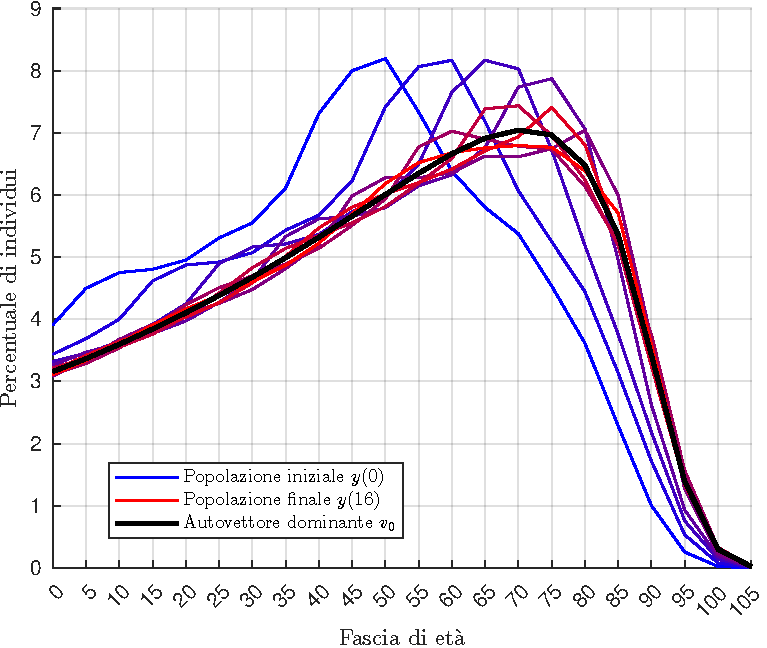
\includegraphics[width=0.9\textwidth]{leslie-dinamica-normalizzata.pdf}
\caption{Percentuale di individui in ogni fascia di età al passare del tempo\\
(incrementi di 10 anni; gradiente di colore da blu a rosso).}
\label{fig:leslie-dinamica-normalizzata}
\end{figure}

\begin{figure}[p]
\centering
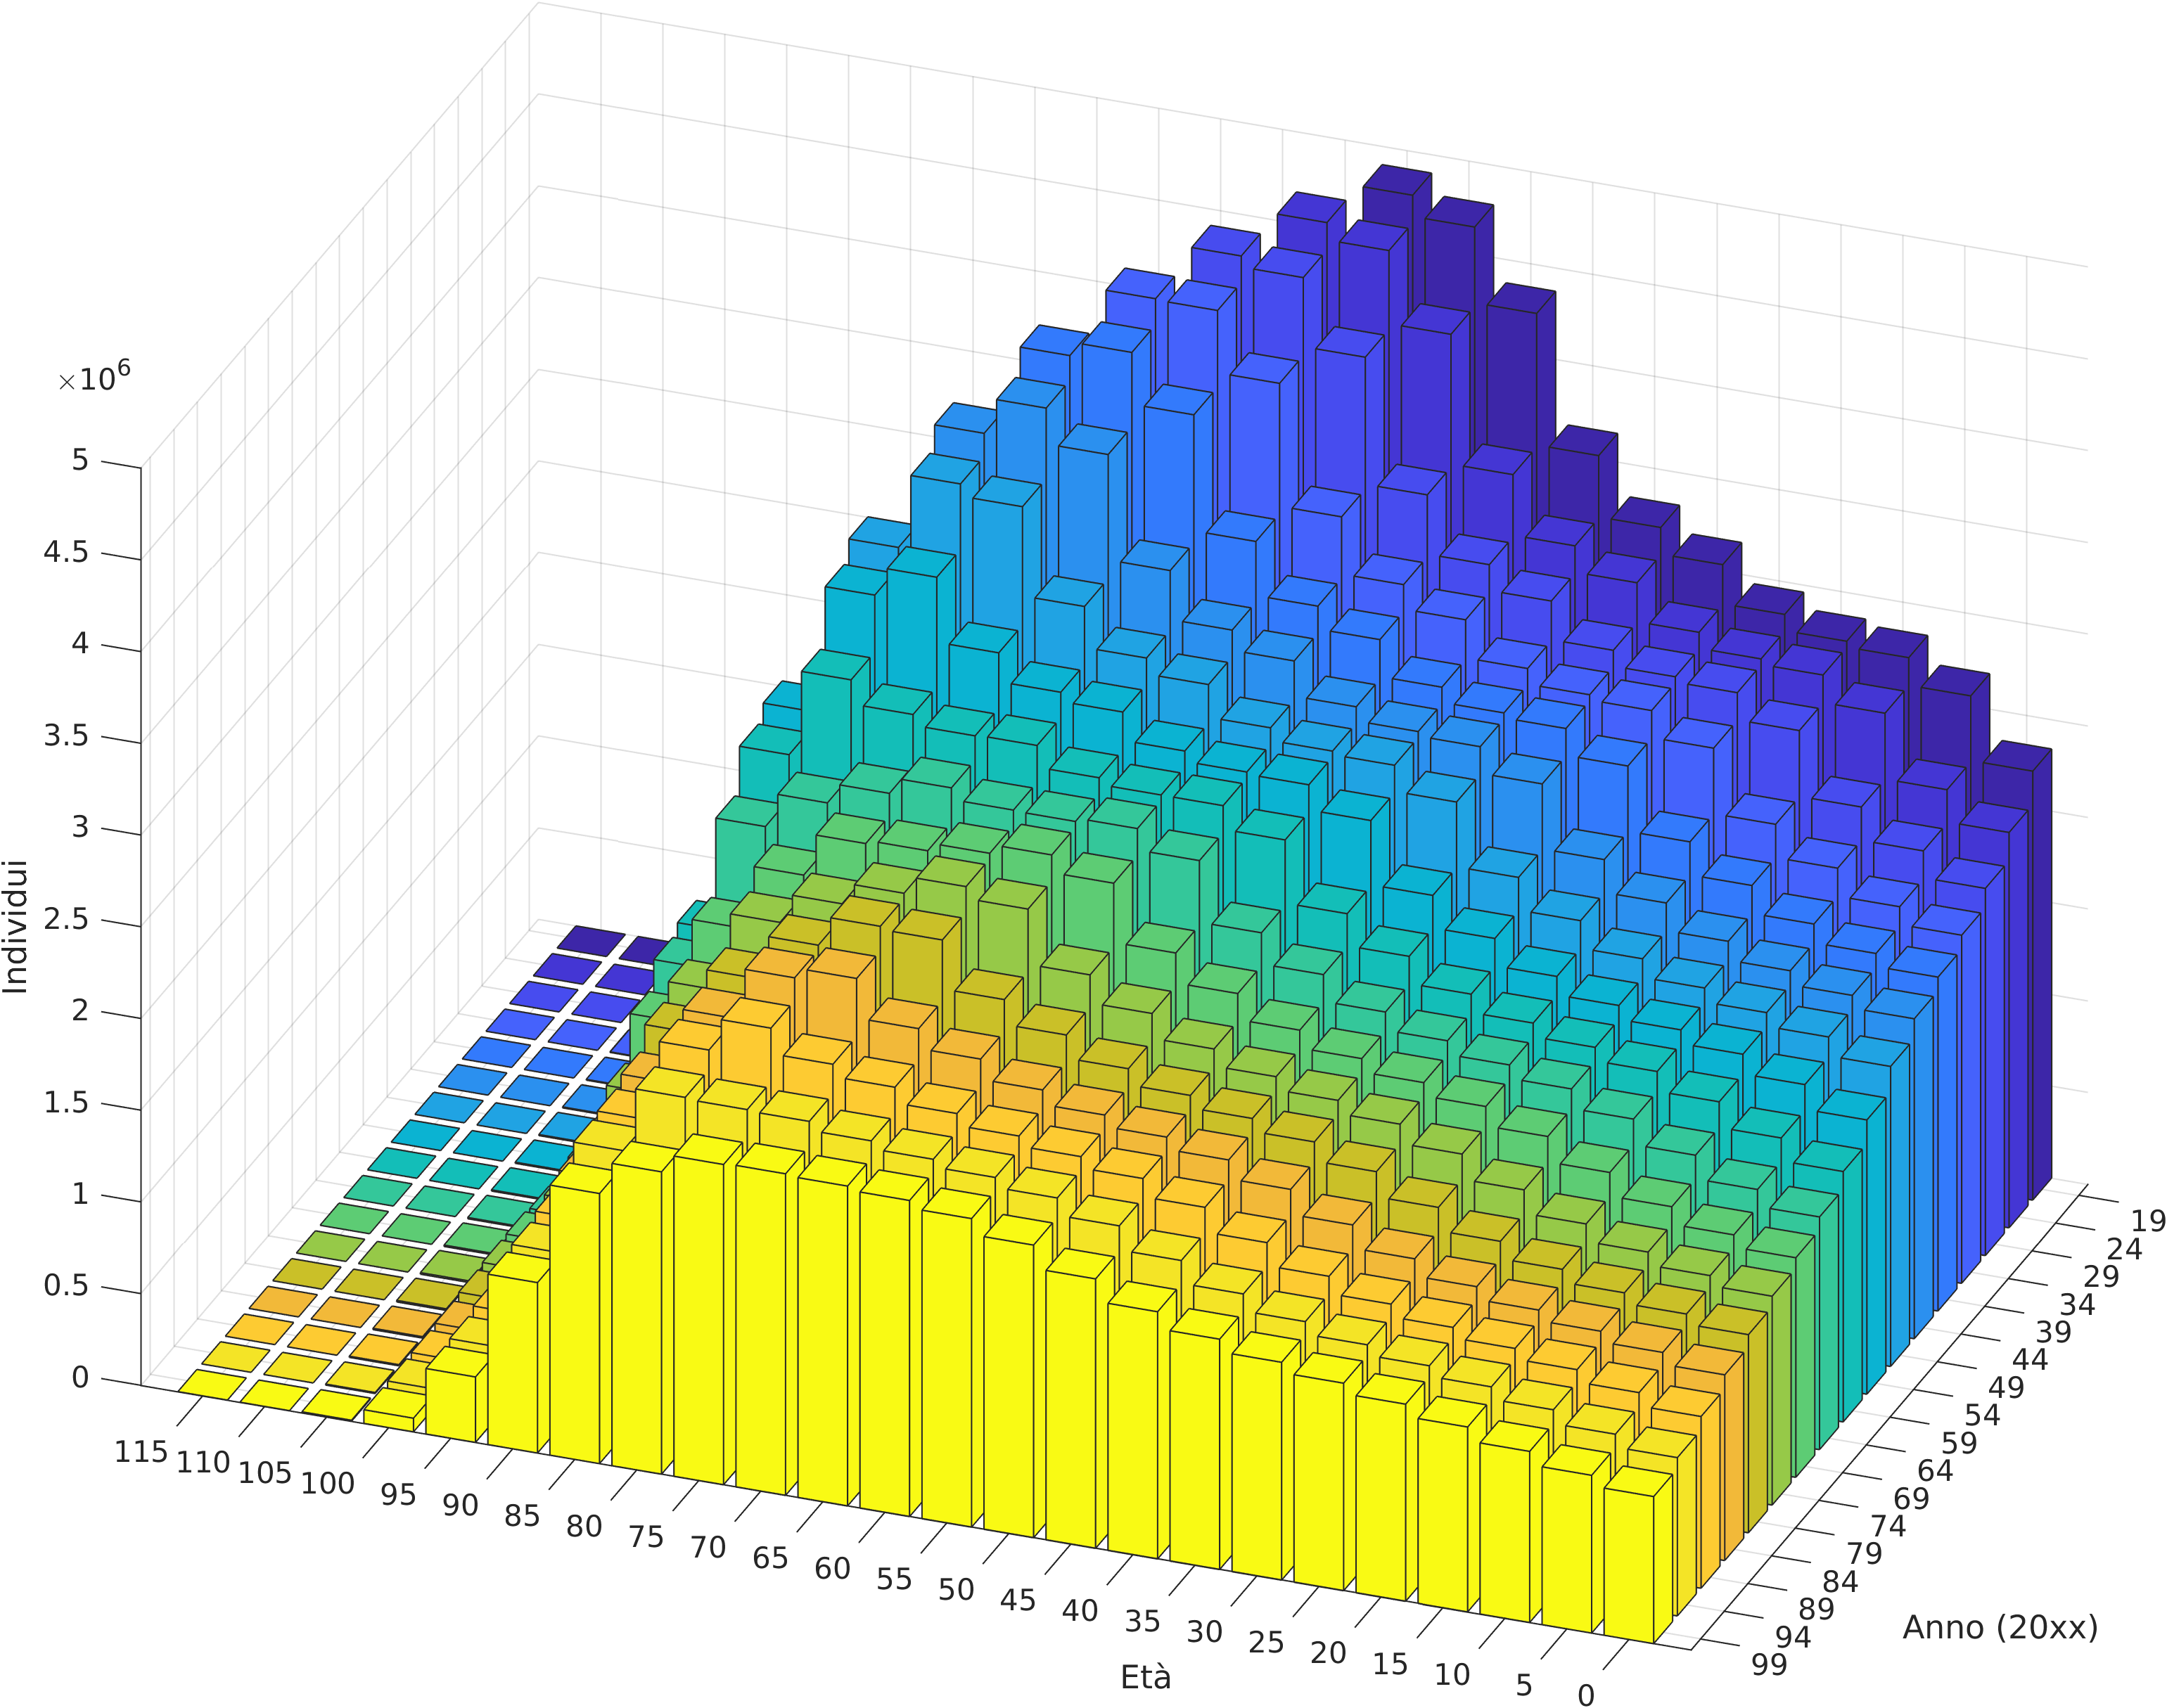
\includegraphics[height=0.45\textheight]{leslie-dinamica-3D-1.png} \\[1em]
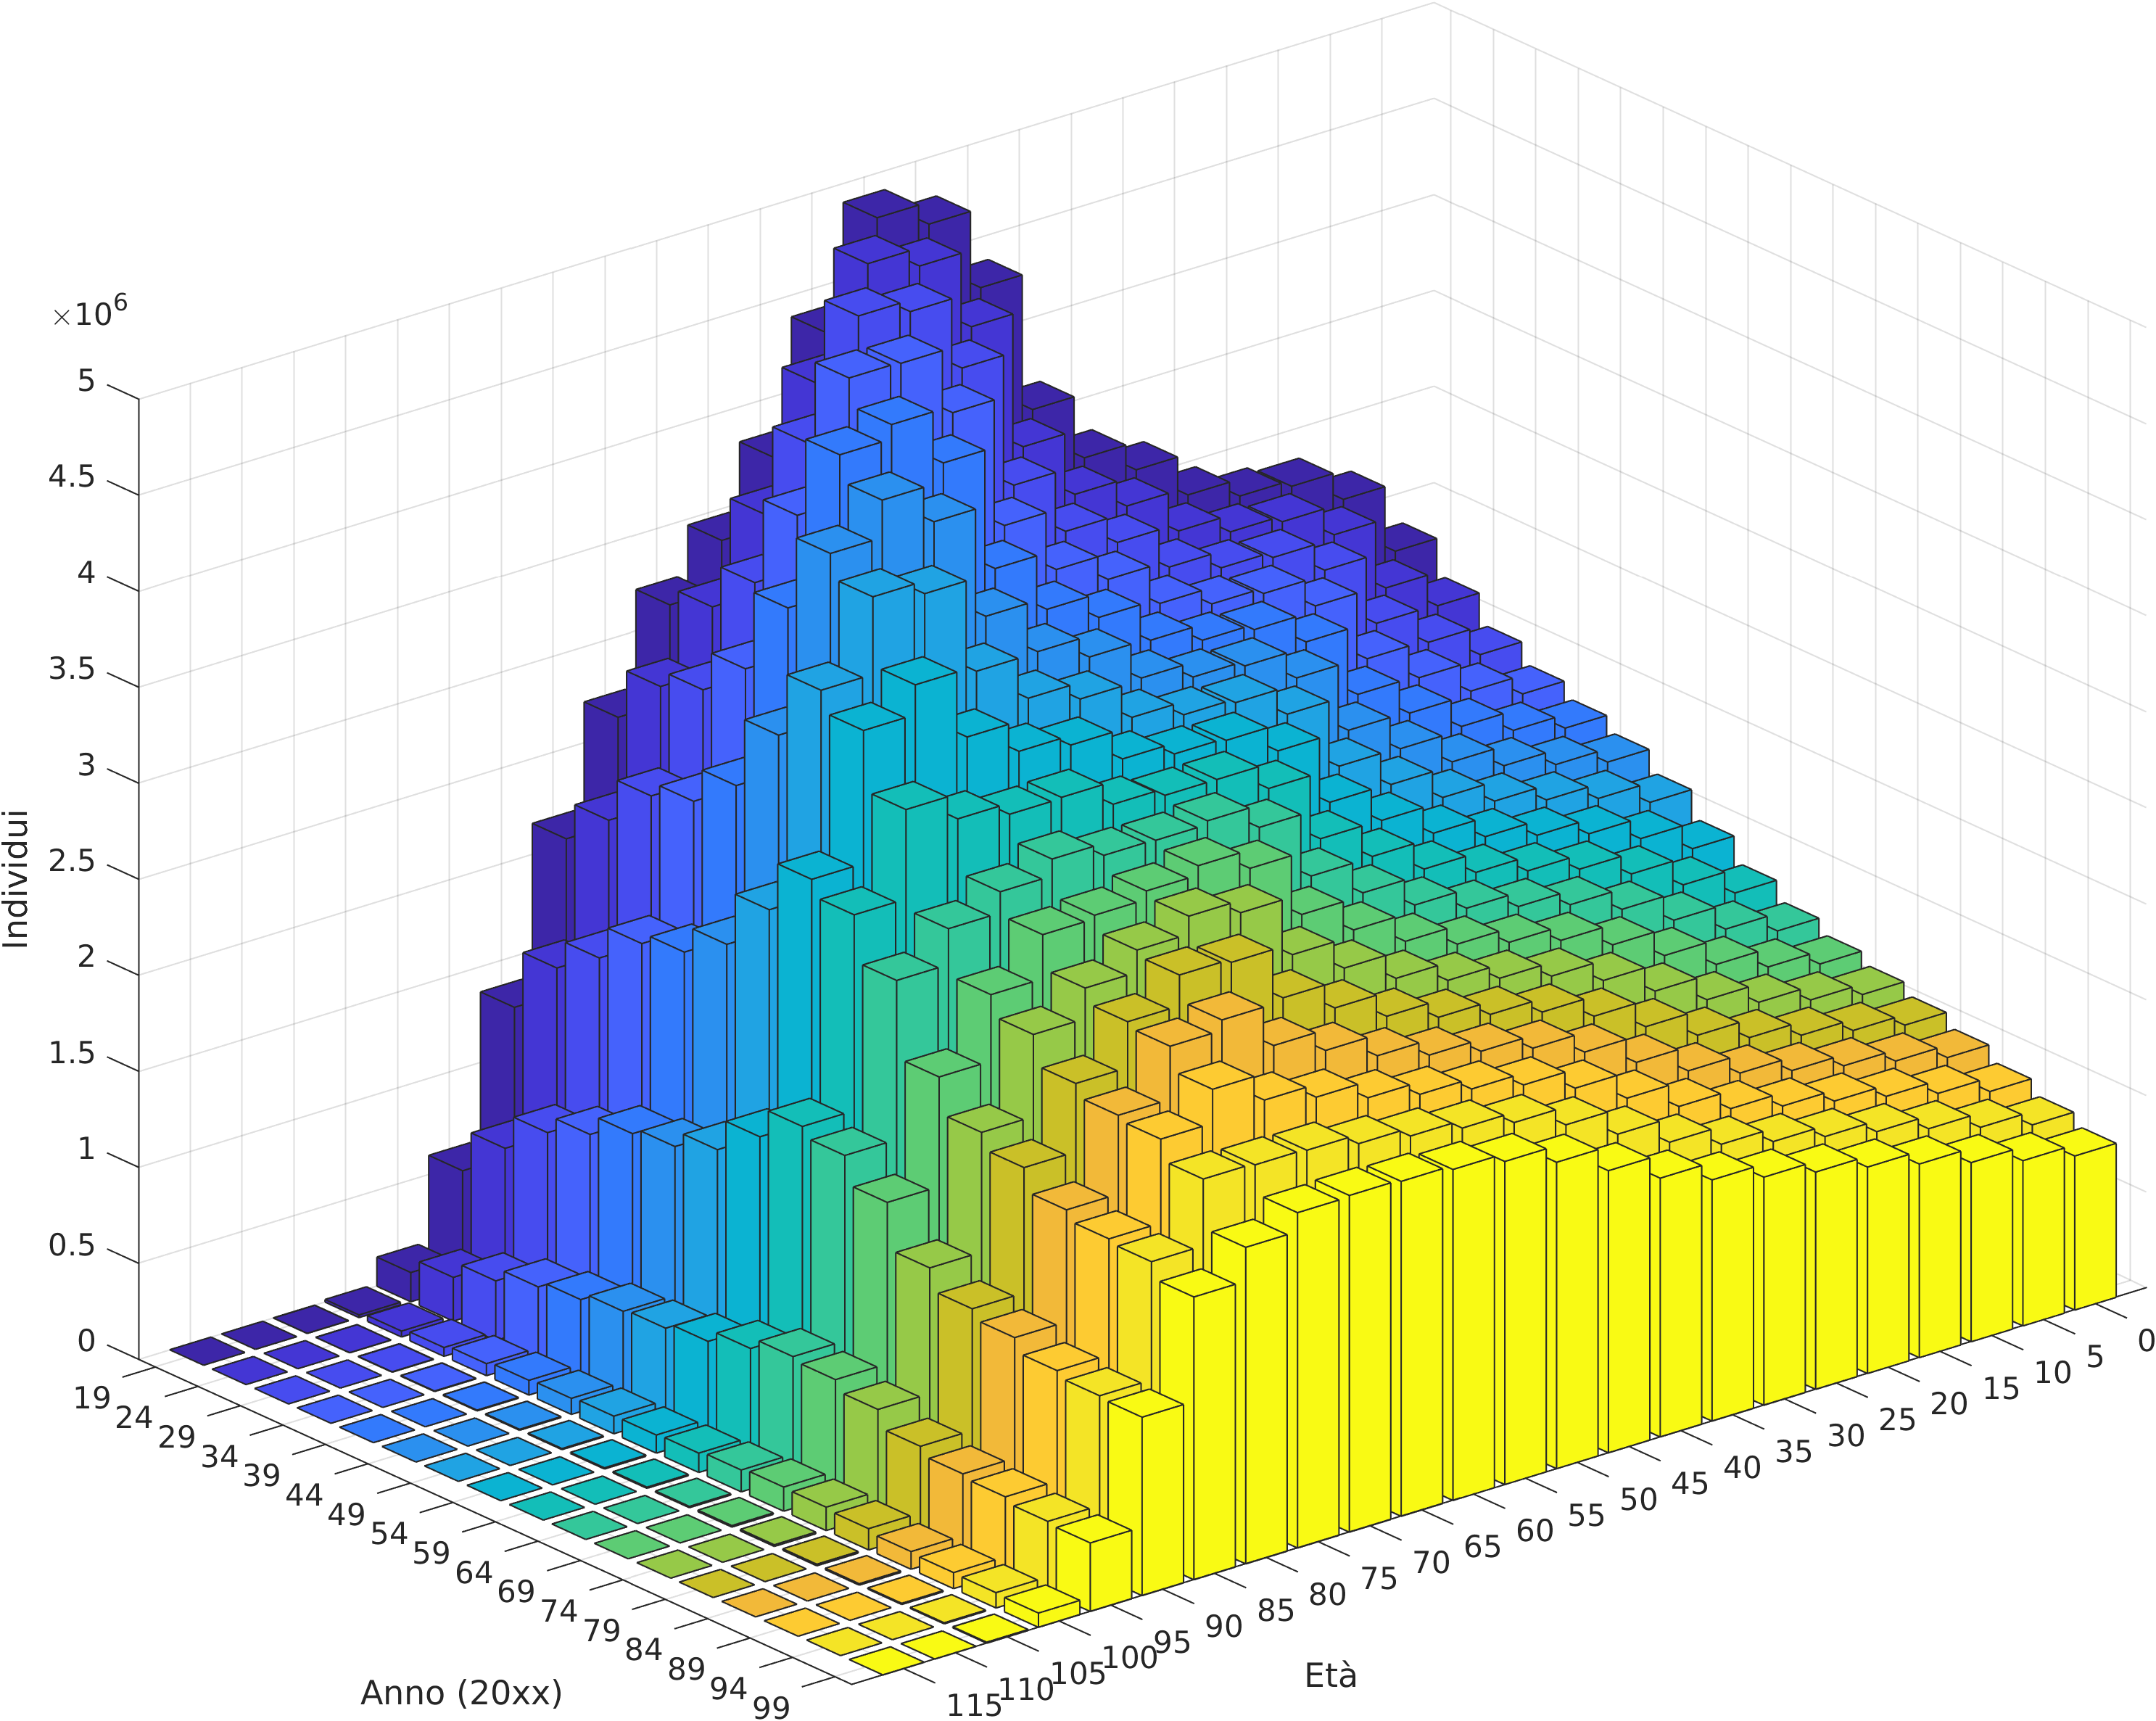
\includegraphics[height=0.45\textheight]{leslie-dinamica-3D-2.png} \vspace{1.5em}
\caption{Dinamica della popolazione italiana nel 21° secolo,
secondo la nostra simulazione.}
\label{fig:leslie-dinamica-3D}
\end{figure}

Dato che la matrice $A$ soddisfa le ipotesi del teorema di Ostrowski,
possiamo andare a verificare che la popolazione si allinei
nella direzione dell'autovettore dominante $v_0$:
la Figura \ref{fig:leslie-dinamica-normalizzata} riporta i vettori
$y(n)$ normalizzati rispetto alla norma 1 (e moltiplicati per 100,
per una maggiore leggibilità), insieme all'autovettore dominante $v_0$ (in nero),
anch'esso normalizzato. In effetti l'allineamento è piuttosto evidente già
dopo 8 iterazioni, cioè nel tempo necessario affinché il picco di individui
tra i 40 e i 60 anni, inizialmente sovrarappresentati, si appiattisca
(tale picco è probabilmente dovuto al fatto che a partire dagli
anni '80 il calo delle nascite è stato molto forte).
L'autovalore dominante $\lambda_0$ di $A$ vale circa 0.935, il che
significa che la popolazione italiana, trascurando gli effetti migratori,
diminuisce di circa il 6.5\% ogni 5 anni.
Questa previsione non è in realtà in buon accordo con quelle dell'ISTAT,
che nelle proprie proiezioni demografiche prospetta un calo della
popolazione assai più contenuto, dell'ordine del 2/3\% secondo
le stime più pessimistiche.
Questa incongruenza è dovuta a diversi fattori, in primis
l'aver trascurato il termine di bilancio migratorio e
l'aver supposto costanti nel tempo i coefficienti $\alpha$ e $\beta$.
Errori minori dovrebbero invece essere associati all'aver aggregato
i dati su base quinquennale e al non aver distinto la dinamica della
popolazione maschile da quella femminile.
%Ad ogni modo, il modello di Leslie è sicuramente migliore di una
%semplice estrapolazione dei dati eseguita in modo indipendente
%su ogni fascia di età, perché quest'ultima non può tenere di conto
%del fenomeno di scorrimento della popolazione dovuto al naturale invecchiamento.

\section{Algoritmo PageRank}

L'algoritmo \emph{PageRank} è una tecnica per l'ordinamento dei nodi
all'interno di una rete (modellata come grafo orientato) in base
alla propria importanza, secondo il criterio per cui
\emph{un nodo è importante se e referenziato da tanti nodi importanti}.
Vista l'enorme applicabilità del concetto di rete, l'algoritmo PageRank
risulta utile nei contesti più disparati (analisi bibliometriche, modelli
cognitivi, classifiche sportive), anche se il più noto è senz'altro quello
dei motori di ricerca: lo stesso nome \emph{PageRank} è un marchio registrato
di Google, che ha impiegato con successo questo algoritmo fin dalla propria
fondazione negli anni '90.

Per poter descrivere il funzionamento dell'algoritmo PageRank, fissiamo
innanzitutto un po' di notazione e introduciamo gli strumenti teorici
necessari. Sia $W = (V,E)$ un grafo orientato (la nostra rete) con insieme
di vertici $V$ (detti anche \emph{nodi}) numerati da 1 a $m \deq \abs{V}$
e con insieme di archi orientati $E$. Se esiste un arco orientato in $E$
che collega due vertici $i,j \in V$ (non necessariamente distinti),
scriveremo che $i \to j$. Per motivi sia teorici che computazionali,
è utile introdurre la \emph{matrice di adiacenza trasposta} del grafo $W$:
\[
L \in \R^{m \times m}, \quad
L_{ij} = \begin{cases}
1 & \text{se $j \to i$},\\
0 & \text{altrimenti}.
\end{cases}
\]
La somma della colonna $i$-esima della matrice $L$ è uguale al numero $f_i$
di archi in uscita dal nodo $i$-esimo, detto \emph{grado in uscita},
mentre la somma della riga $i$-esima di $L$ è uguale al numero di archi
in ingresso al nodo $i$-esimo, detto \emph{grado in entrata}.
Osserviamo che, se non fosse per la possibilità di avere colonne nulle,
la matrice $L$ potrebbe essere normalizzata dividendo ogni colonna per $f_i$,
e si otterrebbe così una matrice stocastica sinistra.
Tale matrice stocastica sarebbe associata alla catena di Markov corrispondente
alla passeggiata aleatoria sul grafo $W$ con probabilità di transizione
uniforme su ogni nodo, ma è chiaro che tale processo stocastico non
può essere ben definito se esistono dei vicoli ciechi, cioè dei nodi senza
archi in uscita. Per rimediare a questo inconveniente, modifichiamo
il grafo $W$ aggiungendo a ogni nodo problematico un collegamento
a tutti i nodi del grafo (tutti, così da non privilegiarne alcuno).
La matrice stocastica sinistra che si ottiene normalizzando $L$
dopo aver modificato $W$ si può dunque scrivere come $S = LF + vd^T$, con
\begin{gather*}
F = \begin{pmatrix}
f_1^\dagger &        &  \\ 
            & \ddots &  \\ 
            &        & f_m^\dagger
\end{pmatrix}, \quad
f_i^\dagger = \begin{cases}
f_i^{-1} & \text{se $f_i > 0$},\\
0        & \text{se $f_i = 0$}
\end{cases}, \quad
e = \begin{pmatrix}
1 \\ \vdots \\ 1
\end{pmatrix} \in \R^m \\
v = \frac{1}{m} e, \quad
d = \begin{pmatrix}
d_1 \\ \vdots \\ d_m
\end{pmatrix}, \quad
d_i = \begin{cases}
1 & \text{se $f_i = 0$},\\
0 & \text{se $f_i > 0$}.
\end{cases}
\end{gather*}
Indichiamo con $y_i$ l'importanza del nodo $i$-esimo della rete $W$,
cioè la grandezza che desideriamo calcolare per mezzo dell'algoritmo PageRank
(e che permette in seguito di ordinare i nodi in base alla loro importanza).
Ovviamente la scala dei valori $y_i$ non è importante: ai fini dell'ordine
conta solo la grandezza relativa.
L'idea alla base dell'algoritmo PageRank può essere formalizzata con il
seguente sistema lineare:
\begin{equation} \label{eq:sistema-lineare-pagerank}
y_i = \sum_{\substack{j = 1,\dots,m \\ L_{ij} \neq 0}} \frac{y_j}{f_j}
\end{equation}
L'importanza del nodo $i$-esimo è infatti espressa come la somma
dell'importanza di tutti i nodi in ingresso, ciascuna pesata
in base al reciproco del grado in uscita (cioè in base all'esclusività
del collegamento). Osserviamo che il sistema lineare \eqref{eq:sistema-lineare-pagerank}
corrisponde al problema agli autovalori $y = Sy$, quindi l'importanza dei nodi
della rete è data dalla distribuzione stazionaria della catena di Markov associata a $S$.
Per il teorema ergodico, tale distribuzione stazionaria è pari al tempo
medio trascorso da una passeggiata aleatoria uniforme su ciascun nodo del grafo;
quest'ultimo punto di vista aiuta a motivare la definizione del PageRank
nel contesto delle ricerche sul web: possiamo pensare a un utente immaginario,
detto \emph{random surfer}, che navighi il web seguendo su ogni pagina
un link in modo casuale tra quelli disponibili con probabilità uniforme,
o che, in assenza di link, ricominci la navigazione da una pagina web casuale.
Allora l'importanza $y_i$ fornita dall'algoritmo PageRank corrisponde
al tempo che il random surfer trascorre in media sulla $i$-esima pagina del web.

Rimangono alcune questioni da sistemare.
Mostriamo innanzitutto che il problema agli autovalori $y = Sy$ ammette
almeno una soluzione:

\begin{teor}
Sia $S = LF + vd^T$. Allora $S \gneq 0$, $e^T S = e^T$ e $\rho(S) = 1$.
\end{teor}

\begin{proof}
Le prime due proprietà sono soddisfatte per costruzione, dunque
$1 \in \sigma(S)$. La terza proprietà segue dal fatto che il raggio
spettrale è maggiorato da una qualsiasi norma matriciale indotta:
\[
1
\leq \rho(S)
\leq \norm{S}_1
= \norm{\smash{e^T S}}_{\infty}
= \norm{\smash{e^T}}_{\infty}
= 1. \qedhere
\]
\end{proof}

\noindent Dunque $\lambda_0 = 1$ è un autovalore dominante di $S$, ma non è
detto che esista un unico autovettore dominante corrispondente.
In generale, infatti, la catena di Markov associata a $S$ può avere
più distribuzioni stazionarie: questo è tipico, per esempio, di quando il grafo
$W$ non è fortemente connesso (perché magari esistono sottoreti isolate,
oppure nodi con un solo arco in uscita verso se stessi, ecc).
Per risolvere questa difficoltà, l'algoritmo PageRank si accontenta
di calcolare l'autovettore dominante della matrice
\[
pS + (1-p) \frac{1}{m} e \, e^T, \quad p \in (0,1),
\]
che per valori di $p$ vicini a 1 è vicina a $S$, ma allo stesso tempo
è strettamente positiva: in questo modo è possibile applicare il teorema
di Perron-Frobenius in forma forte, e questo garantisce che l'autovettore
dominante $v_0$ sia unico (a meno di una costante positiva, ovviamente).
Osserviamo che $v_0$ può essere pensato come il punto di equilibrio
del seguente sistema dinamico discreto:
\[
\left\{
\begin{aligned}
& y(n+1) = \Bigl( pS + (1-p) \frac{1}{m} e \, e^T \Bigr) y(n) \quad \forall n \geq 0, \\
& y(0) = y_0 \in \R^m.
\end{aligned}
\right.
\]
Dato che si può dimostrare che $e^T y(n) = e^T y_0$, tale sistema può essere scritto
in forma non omogenea come
\begin{equation} \label{eq:sistema-dinamico-pagerank}
\left\{
\begin{aligned}
& y(n+1) = p S y(n) + (1-p) \frac{1}{m} e \norm{y_0}_1 \quad \forall n \geq 0, \\
& y(0) = y_0 \in \R^m.
\end{aligned}
\right.
\end{equation}
Il raggio spettrale della matrice $pS$ è $p < 1$, quindi il Teorema \dots
ci conferma che esiste ed è unico un punto di equilibrio $v_0$,
che $v_0 > 0$ è asintoticamente stabile e che
\[
y(n) = (pS)^n (y_0 - v_0) + v_0.
\]
Quest'ultima formula ci permette di concludere non solo che $y(n) \to v_0$,
ma anche che l'errore $\norm{y(n)-v_0}_1$ tende a zero come
$\norm{pS}_1^n = p^n$.
Dunque l'iterazione \ref{eq:sistema-dinamico-pagerank} fornisce un metodo
efficace per il calcolo di $v_0$, senza ricorrere ad algoritmi di algebra
lineare densa che richiederebbero troppo tempo e troppa memoria nel caso
del web o di altre reti con miliardi di nodi. Osserviamo che valori
di $p$ più vicini a 1 permettono di mantenersi più fedeli alla rete originale
$W$ e alla passeggiata aleatoria su di essa definita, mentre valori di $p$
più vicini a zero permettono di convergere più velocemente a $v_0$
per mezzo del metodo iterativo appena esposto. Nella pratica, l'evidenza empirica
suggerisce che valori intorno a 0.85 siano un buon compromesso.

\subsection*{PageRank del sito web del CNR}

Vediamo ora come l'algoritmo PageRank possa essere applicato all'analisi di
una rete reale, per esempio quella formata da tutte le pagine web di un
dato sito. Mediante una ricerca su Google (per l'appunto), abbiamo trovato un
dataset interessante, elaborato dal Laboratory for Web Algorithmics
dell'Università degli studi di Milano e pubblicato alla pagina
\url{http://law.di.unimi.it/webdata/cnr-2000/}.
Il dataset consiste in una scansione completa del sito del
Centro Nazionale di Ricerca italiano (CNR), effettuata nell'anno 2000
e contenente circa $3 \cdot 10^5$ nodi e $3 \cdot 10^6$ collegamenti
(tutti i link esterni al dominio \url{cnr.it} sono stati rimossi).
Sul sito del Laboratory for Web Algorithmics il grafo $W$ è stato pubblicato
in un formato compresso pensato per l'elaborazione con il framework WebGraph
(sviluppato dallo stesso laboratorio di ricerca), tuttavia sul sito
\url{sparse.tamu.edu} è possibile scaricare la matrice di adiacenza (non trasposta)
del grafo $W$ direttamente in formato \code{.mat}, quello nativo di MATLAB.
Sulla pagina del Laboratory for Web Algorithmics sono inoltre riportate
le etichette del dataset, cioè le stringhe $s_i$ che contengono l'url
del nodo $i$-esimo, indispensabili per interpretare il risultato
dell'algoritmo.

Il Programma \ref{prog:pagerank} contiene il codice che abbiamo utilizzato
per calcolare il PageRank del sito web del CNR tramite l'algoritmo
iterativo con $p = 0.85$ visto in precedenza. Le 20 pagine web più importanti
sono riportate nella Tabella \ref{tab:pagerank}, insieme ai loro indici
$i$ all'interno del dataset e i loro valori $y_i$
(il vettore $y$ è normalizzato in modo da avere somma 1).
Osserviamo che il numero di iterazioni \code{nmax} è stato scelto in modo
da garantire un errore su $y(\text{\code{nmax}})$ dell'ordine di $10^{-6}$, che ci è
sembrato più che sufficiente a fronte di un grafo con $3 \cdot 10^5$ nodi
(perché ci basta distinguere i valori $y_i$ dei nodi più importanti).
Nel Programma \ref{prog:pagerank} abbiamo fatto attenzione a preservare
la sparsità di $L$, in particolar modo evitando di formare la matrice
$S = LF + vd^T$ (potenzialmente densa). In questo modo, l'algoritmo PageRank
richiede soltanto $O(m)$ memoria e $O(m)$ operazioni aritmetiche: per questo
è possibile calcolare il PageRank anche di grafi enormi, come fa Google con il web.

\lstinputlisting[float=p, label=prog:pagerank, caption={Applicazione
dell'algoritmo PageRank all'analisi del sito web del CNR.}]{pagerank.m}

\pgfplotstableset{
	columns/rank/.style={int detect, column name={Rank}},
	columns/url/.style={column type=l, string type, column name={URL}},
	columns/i/.style={int detect, 1000 sep={}, column name=$i$},
	columns/y/.style={column name=$y_i$}
}

\begin{table}[p]
\caption{PageRank del dataset relativo al sito web del CNR nell'anno 2000.}
\label{tab:pagerank}
\centering
\pgfplotstabletypeset{pagerank-pulito.dat}
\end{table}

\section{Modello di corsa agli armamenti}

Vediamo infine un esempio di sistema dinamico positivo continuo.
Il \emph{modello di corsa agli armamenti} fu introdotto dal matematico inglese
Lewis Fry Richardson (noto anche per la tecnica di estrapolazione)
per descrivere l'evoluzione nel tempo dei livelli di armamento $y_i(t)$
di due o più nazioni in competizione militare tra loro, sotto l'ipotesi che
la variazione $y'_i(t)$ di ciascun livello di armamento sia influenzata in modo
positivo dai livelli di armamento $y_j(t)$ raggiunti dalle nazioni avversarie
e in modo negativo dal livello di armamento $y_i(t)$ già raggiunto dalla
propria nazione, secondo il principio per cui mantenere un esercito grande
è molto costoso, ma allo stesso tempo nessuna nazione desidera avere un esercito
inferiore a quello dei propri avversari. Formalmente, nel caso di due
nazioni, il modello consiste nel sistema dinamico lineare
\[
y'(t) =
\begin{pmatrix*}[r]
-a & b \\
c & -d
\end{pmatrix*}
y(t) +
\begin{pmatrix}
\xi_0 \\
\eta_0
\end{pmatrix}
\qquad a,b,c,d, \xi_0, \eta_0 > 0.
\]
I coefficienti $a$ e $d$ sono detti \emph{coefficienti di affaticamento}
e corrispondono al tasso di decrescita dei livelli di armamento in assenza di
competizione, mentre i coefficienti $b$ e $c$ sono detti \emph{coefficienti
di competizione} e corrispondono al tasso di crescita dei livelli di armamento
che si avrebbe se le spese di mantenimento degli eserciti fossero nulle.
Infine, i coefficienti $\xi_0$ e $\eta_0$ corrispondono a dei valori
basali dovuti alla naturale tendenza delle popolazioni umane ad armarsi,
aldilà degli effetti dovuti all'affaticamento o alla competizione.

Cerchiamo ora di capire quali sotto quali condizioni sui coefficienti
del modello si possa avere una coesistenza pacifica delle nazioni, cioè esista
un punto di equilibrio $\bar{y}$ asintoticamente stabile (viceversa, una
\emph{corsa agli armamenti}, cioè una crescita incontrollata dei livelli
$y_1(t)$ e $y_2(t)$, porterebbe a una guerra). Osserviamo che
\[
A = \begin{pmatrix*}[r]
-a & b \\
c & -d
\end{pmatrix*}
= \begin{pmatrix*}[c]
-a +\alpha & \hspace{0.7em} b \\
\hspace{0.65em} c & -d + \alpha
\end{pmatrix*}
- \alpha	 I
\]
è una matrice di Metzler, se $\alpha > \max\{a,d\}$. Allora, abbiamo una
conferma che il sistema dinamico è positivo, e possiamo quindi applicare
il Teorema \ref{teor:equilibrio-sistema-dinamico-positivo-continuo},
per cui esiste un punto di equilibrio $\bar{y}$ strettamente positivo
se e solo se $\sigma(A) \subseteq \C^-$.
Dato che $m = 2$, è possibile esprimere in modo semplice il valore di $\bar{y}$
in funzione dei coefficienti del modello per mezzo della regola di Cramer:
\[
\bar{y_1} = \frac{\xi_0 d + b \eta_0}{ad-bc}
\quad \bar{y_2} = \frac{a \eta_0 + \xi_0 c}{ad-bc}.
\]
Osserviamo dunque che $\bar{y} > 0$ se e solo se $ad-bc > 0$.
Allora, per il Teorema \ref{teor:equilibrio-sistema-dinamico-positivo-continuo}
si ha che la dinamica del modello è asintoticamente stabile se e solo se
$ad > bc$, cioè se e solo se il prodotto dei coefficienti di affaticamento
è maggiore del prodotto dei coefficienti di competizione.
A conclusione di questo paragrafo, abbiamo simulato due dinamiche di esempio,
una stabile (Figura \ref{fig:corsa-agli-armamenti-1}) e una instabile
(Figura \ref{fig:corsa-agli-armamenti-2}). Nel primo caso,
\[
a = 1.2, \quad b = 1, \quad c = 1, \quad d = 1.2,
\quad \xi_0 = 1, \quad \eta_0 = 2, \quad t \in [0,15], \quad y_0 = (0.5,5)^T,
\]
quindi $ad = 1.44 > 1 = bc$ e si ha $y(t) \to \bar{y} \approx (7.27,7.73)^T$,
mentre nel secondo caso
\[
a = 0.9, \quad b = 2, \quad c = 1, \quad d = 2,
\quad \xi_0 = 1, \quad \eta_0 = 2, \quad t \in [0,10], \quad y_0 = (0.5,5)^T,
\]
quindi $ad = 1.8 < 2 = bc$ e si ha $\norm{y(t)} \to +\infty$.
Le due simulazioni sono state effettuate tramite il Programma \ref{prog:corsa-agli-armamenti},
che risolve il sistema di equazioni differenziali con il metodo dei trapezi
(implementato come metodo di Adams-Moulton a un passo) e passo temporale $h = 0.1$.

\begin{figure}[!b]
\centering
\begin{tikzpicture}[trim axis left]
\begin{axis}[
	xlabel={$t$},
	ylabel={$y(t)$},
	legend style={anchor=south east,at={(0.96,0.06)}},
	xmin = -0.5, xmax = 15.5,
	width=0.9\textwidth,
	height=0.35\textheight
]
\addplot[red] table[x=t, y=y1] {corsa-agli-armamenti-1.dat};
\addplot[blue] table[x=t, y=y2] {corsa-agli-armamenti-1.dat};
\legend{$y_1(t)$, $y_2(t)$}
\end{axis}
\end{tikzpicture}
\caption{Esempio di dinamica stabile del modello di corsa agli armamenti.}
\label{fig:corsa-agli-armamenti-1}
\end{figure}

\begin{figure}[p]
\centering
\begin{tikzpicture}[trim axis left]
\begin{axis}[
	xlabel={$t$},
	ylabel={$y(t)$},
	legend style={anchor=south east,at={(0.96,0.06)}},
	xmin = -0.5, xmax = 10.5,
	width=0.9\textwidth,
	height=0.35\textheight
]
\addplot[red] table[x=t, y=y1] {corsa-agli-armamenti-2.dat};
\addplot[blue] table[x=t, y=y2] {corsa-agli-armamenti-2.dat};
\legend{$y_1(t)$, $y_2(t)$}
\end{axis}
\end{tikzpicture}
\caption{Esempio di dinamica instabile del modello di corsa agli armamenti.}
\label{fig:corsa-agli-armamenti-2}
\end{figure}

\lstinputlisting[float=p, label=prog:corsa-agli-armamenti, caption={Simulazione
del modello di corsa agli armamenti: caso stabile e caso instabile.}]
{figures_corsa_agli_armamenti.m}
